\begin{frame}{Existing panels and screens provide the BDE reference}
  \begin{columns}[T,onlytextwidth]
    \begin{column}{0.47\textwidth}
      \textbf{TPC protection panel designs}\par\medskip
      \includegraphics[page=2,width=\linewidth,height=3.1cm,keepaspectratio,
        trim=290bp 500bp 900bp 430bp,clip]{figures/tpc-panel-reference.pdf}\par
      \medskip\captionline{Central PLC, bias I/O and LV/fan/heater reference panels.}
    \end{column}
    \begin{column}{0.49\textwidth}
      \textbf{BDE Ignition screens}\par\medskip
      \includegraphics[page=7,width=\linewidth,height=3.1cm,keepaspectratio,
        trim=10bp 210bp 460bp 74bp,clip]{figures/sc-progress-june2026.pdf}\par
      \captionline{Existing Ignition display of the BDE crate groups.}
    \end{column}
  \end{columns}\par
  \medskip
  Parts list: CX5140 PLC, EK1100 couplers, EK1521 fibre links and EL2124 inhibit outputs.\par\medskip
  \raggedright\DuneDiagramCaption{Reference panel design and existing operator screen. The VD group contains eight warm crates.}
\end{frame}

\begin{frame}{The fan trip removes the PL506 channel permit}
  \centering
  \begin{tikzpicture}[
    box/.style={draw=DuneTextMuted,fill=none,text=DuneText,align=center,
      text width=1.75cm,minimum height=1.25cm,inner sep=4pt,font=\small},
    edge/.style={-{Stealth},draw=DuneTextMuted,line width=1.2pt}]
    \node[box] (fan) at (-5.75,0.6) {Fan status\\DB25 cable};
    \node[box] (input) at (-3.45,0.6) {EL1004\\input I/O};
    \node[box,fill=none] (plc) at (-1.15,0.6) {DPS PLC\\cooling rule};
    \node[box] (output) at (1.15,0.6) {EL2124\\5 V output};
    \node[box,fill=none] (supply) at (3.45,0.6) {PL506\\channel inhibit};
    \node[box] (load) at (5.75,0.6) {Affected WIEC\\48 V feed};
    \draw[edge] (fan) -- (input);
    \draw[edge] (input) -- (plc);
    \draw[edge] (plc) -- (output);
    \draw[edge] (output) -- (supply);
    \draw[edge] (supply) -- (load);
    \node[font=\small] at (-2.3,1.55) {EtherCAT};
    \node[font=\small] at (0,1.55) {EtherCAT};
    \node[font=\small] at (2.3,1.55) {Wired};
  \end{tikzpicture}\par
  \medskip
  \raggedright\DuneDiagramCaption{Cooling fault $\rightarrow$ withdraw the permit for the affected PL506 channel.}
  \medskip
  \raggedright \textbf{Feedback:} PL506 state and voltage/current $\rightarrow$ SNMP $\rightarrow$ DPS;
  OPC UA carries the result to SC for logging.\par
  \medskip
  \textbf{VD allocation check:} six fan-status signals per WIEC means 48 per
  eight-WIEC group. Match these to the populated VD inputs and cables.\par
  \captionline{Six fans per crate is the design case used here. These are existing input requirements, not additional I/O.}
\end{frame}

\begin{frame}{DAQ CCM and Hermes use distinct DAPHNE services}
 \centering
 \begin{adjustbox}{max width=\linewidth}% Adapted from icd-sc-pds/sections/03_protocols_services.tex at bfb2a8b.
\begin{tikzpicture}[
 box/.style={draw=DuneTextMuted,fill=none,text=DuneText,align=center,font=\small,inner sep=5pt},
 flow/.style={-{Stealth},draw=DuneTextMuted,line width=1pt},
 both/.style={arrows={Stealth-Stealth},draw=DuneTextMuted,line width=1pt}]
\node[box,text width=37mm] (ignition) at (0,0)
 {SC server\\OPC UA client $\rightarrow$ Ignition};
\node[box,text width=32mm] (daq) at (5.0,0) {DAQ CCM client\\opmon subscriber};
\node[box,text width=35mm] (hermesclient) at (10.7,0)
 {DAQ Hermes\\configuration client};
\node[box,text width=75mm,minimum height=13mm] (ua) at (2.5,-1.8)
 {SC bridge server\\ZMQ client $\rightarrow$ OPC UA bridge\\Integrated DAQ configuration};
\node[box,text width=65mm,minimum height=12mm] (daphne) at (2.5,-4)
 {DAPHNE\\AXI / OS $\rightarrow$ daphne-server $\rightarrow$ ZMQ};
\node[box,text width=37mm,minimum height=15mm] (hermes) at (10.7,-4)
 {Board-side Hermes\\IPBus / UDP\\Configuration endpoint};
% An open bracket groups board services without crossing the exchange labels.
\node[fit=(daphne)(hermes),inner sep=8pt,
 label={[font=\small,text=DuneTextMuted]below:One DAPHNE board; one shared 1\,Gb Ethernet CCM connection}] (board) {};
\draw[draw=DuneTextMuted,dashed] (board.north west) -- (board.south west)
  -- (board.south east) -- (board.north east);
\draw[both] (ignition) -- node[left,font=\small]{OPC UA} (ignition |- ua.north);
\draw[both] (daq) -- node[right,font=\small]{OPC UA} (daq |- ua.north);
\draw[both] ([xshift=-11mm]ua.south) -- node[left,align=right,font=\small,inner sep=2pt]
 {Configuration\\request/response} ([xshift=-11mm]daphne.north);
\draw[flow] ([xshift=11mm]daphne.north) -- node[right,align=left,font=\small,inner sep=2pt]
 {Published\\monitoring} ([xshift=11mm]ua.south);
\draw[both] (hermesclient.south) -- node[right,align=left,font=\small]
 {IPBus / UDP\\configuration} (hermes.north);
\end{tikzpicture}
\end{adjustbox}\par
 \raggedright\DuneDiagramCaption{Working SC--PDS--DPS ICD, Figure 1. DAQ CCM/opmon and Hermes remain distinct clients. The dashed bracket groups the board-side services.}
\end{frame}

\begin{frame}{Rack space is not a count of spare I/O terminals}
  \renewcommand{\arraystretch}{1.4}
  \begin{tabularx}{\textwidth}{@{}>{\RaggedRight\arraybackslash}p{3.4cm}r>{\RaggedRight\arraybackslash}X@{}}
    \toprule
    \textbf{Rack type} & \textbf{Count} & \textbf{DPS allocation and workbook space}\\
    \midrule
    BDE auxiliary & 10 & 12U DPS; U3--U21 marked Space (19U); eight WIECs per rack\\
    BDE low voltage & 20 & One PL506 per rack; four WIECs per supply\\
    Bias high voltage & 10 & 12U DPS; U3--U12 marked Space (10U)\\
    \bottomrule
  \end{tabularx}\par
  \bigskip
  Space marked in the rack workbook is not a new DPS reservation.
  Free DIN-rail length and I/O capacity depend on the populated VD panel.
  \captionline{U denotes rack height. The marked space is not an allocation of free PLC terminals.}
\end{frame}

\begin{frame}{The bias draft provides 1,440 outputs for review}
  \renewcommand{\arraystretch}{1.3}
  \begin{tabularx}{\textwidth}{@{}>{\RaggedRight\arraybackslash}Xrr@{}}
    \toprule
    \textbf{Component} & \textbf{Per rail} & \textbf{10 racks}\\
    \midrule
    EK1100 EtherCAT coupler & 1 & 20\\
    EL9410 supply terminal & 1 & 20\\
    EL2124: four 5 V outputs & 18 & 360\\
    EL9011 end cap & 1 & 20\\
    24 V power supply & 1 & 20\\
    \bottomrule
  \end{tabularx}\par
  \medskip
  Each rail occupies 337 mm. The draft provides 1,440 output channels;
  the working VD inventory lists 576 bias channels.\par
  \captionline{Draft layout: the difference between 1,440 outputs and 576 bias channels is not verified spare capacity.}
\end{frame}

\begin{frame}{Supply capacity differs from expected power use}
  \small
  \renewcommand{\arraystretch}{1.3}
  \begin{tabularx}{\textwidth}{@{}>{\RaggedRight\arraybackslash}p{3.7cm}>{\RaggedRight\arraybackslash}p{2.4cm}>{\RaggedRight\arraybackslash}X@{}}
    \toprule
    \textbf{Equipment} & \textbf{Power / capacity} & \textbf{Basis and limit}\\
    \midrule
    PL506 input & 2.25 kW each & 20 supplies: about 45.1 kW expected AC input\\
    WIEC fans only & 380 W per group & $8\times6\times0.33\,\mathrm{A}\times24\,\mathrm{V}$; excludes heaters and I/O\\
    Bias DPS supply allowance & 24 V, 40 A & 960 W DC capacity per rack in the workbook\\
    \bottomrule
  \end{tabularx}\par
  \medskip
  The inherited 831 W auxiliary figure needs a VD component budget
  covering fans, heaters and populated I/O.\par
  \captionline{Fan power assumes six fans per crate. Supply capacity is distinct from expected consumption.}
\end{frame}

\begin{frame}{Map each rack package against the existing allowance}
  \small
  \renewcommand{\arraystretch}{1.2}
  \begin{tabularx}{\textwidth}{@{}>{\RaggedRight\arraybackslash}p{3.4cm}>{\RaggedRight\arraybackslash}X@{}}
    \toprule
    \textbf{Rack component} & \textbf{Reference hardware / allocation}\\
    \midrule
    PDU & Raritan PX3; inlet and outlet allocation for the connected loads\\
    Smoke detector & 4WTAR-B and EOLR-1 end-of-line relay\\
    Contact interface & DX-PD2C5; 12 V supply to the smoke detector\\
    Humidity & Record the probe and peripheral interface for each rack\\
    Temperature / water leak & PDU peripheral sensors where fitted\\
    \bottomrule
  \end{tabularx}\par
  \medskip
  \normalsize The May workbook includes a 76-entry rack-protection/PDU allowance.
  Map the actual rack packages against this existing allowance.\par
  \captionline{Humidity probe models and any humidity-trip requirement remain to be specified.}
\end{frame}

\begin{frame}{Local PDU trips need deliberate power restoration}
  \renewcommand{\arraystretch}{1.45}
  \begin{tabularx}{\textwidth}{@{}>{\RaggedRight\arraybackslash}p{3.7cm}>{\RaggedRight\arraybackslash}X@{}}
    \toprule
    \textbf{PX3 setup guide} & \textbf{Local behaviour documented}\\
    \midrule
    Smoke, water, temperature & Local event rules and scripts can switch off the protected outlets\\
    Network-switch outlet & Kept powered during the guide's fallback shutdown\\
    After a local trip & Power is restored deliberately; no automatic restoration\\
    \bottomrule
  \end{tabularx}\par
  \bigskip
  The VD control chain is Ignition $\rightarrow$ DPS PLC $\rightarrow$ PDU.
  Local trip status returns to the PLC and to SC for logging.
  \captionline{The reference prototype used direct Ignition control. The VD PLC path still needs its own communication-loss and recovery tests.}
\end{frame}

\begin{frame}{Keep subsystem quantities separate from crate totals}
  \renewcommand{\arraystretch}{1.35}
  \begin{tabularx}{\textwidth}{@{}>{\RaggedRight\arraybackslash}p{3.2cm}>{\RaggedRight\arraybackslash}X@{}}
    \toprule
    \textbf{Subsystem} & \textbf{Working inventory and interfaces}\\
    \midrule
    PDS readout / calibration & 34 LV feeds in the current presentation scope; supply status and control interfaces\\
    Power over fibre (PoF) & 80 boxes; 320 voltage and 80 temperature readings; Opta PLC or Beckhoff PLC alternative\\
    TDE & 20 mezzanine racks; DPS controls PDUs; crate-status and external-inhibit interfaces remain options\\
    Calibration / cryogenic instrumentation & Level and temperature readout, purity monitors, ionization laser and neutron source\\
    \bottomrule
  \end{tabularx}
  \captionline{TDE and DAQ/timing contain 336 microTCA crates in total. Crate totals do not establish the number of PDUs or network switches.}
\end{frame}

\begin{frame}{Survey the 20 panel references to find installed hardware}
  \renewcommand{\arraystretch}{1.4}
  \begin{tabularx}{\textwidth}{@{}>{\RaggedRight\arraybackslash}p{3.4cm}>{\RaggedRight\arraybackslash}X@{}}
    \toprule
    \textbf{Drawing area} & \textbf{Interfaces on the inspection maps}\\
    \midrule
    CUC, level 4850 & Eight panel references: air handling, chilled water, power and associated equipment\\
    Level 4910 & North and south sump interfaces, SP-1 and SP-2\\
    4850-08-ES group & Spare panel for future equipment; mapped to the access-drift inspection area\\
    Other 4850 areas & Chillers, pumps, ventilation and generator interfaces\\
    \bottomrule
  \end{tabularx}\par
  \medskip
  Marked inspection maps cover the 4850 and 4910 levels.
  \captionline{These are drawing references. The underground survey will establish what is installed.}
\end{frame}

\begin{frame}{The workbook allocates 76 mezzanine rack positions}
  \renewcommand{\arraystretch}{1.15}
  \begin{tabularx}{\textwidth}{@{}>{\RaggedRight\arraybackslash}Xr>{\RaggedRight\arraybackslash}Xr@{}}
    \toprule
    \textbf{Rack type} & \textbf{Count} & \textbf{Rack type} & \textbf{Count}\\
    \midrule
    BDE low voltage & 20 & PDS low voltage & 4\\
    BDE auxiliary & 10 & Drift HV & 2\\
    TDE & 20 & Reserved drift HV & 2\\
    Bias HV & 10 & Spare / CalCI & 8\\
    \bottomrule
  \end{tabularx}\par
  \bigskip
  \textbf{76 numbered mezzanine positions:} SEDM-01 to SEDM-76.\par
  \medskip
  The worksheet also has a separate concept for 40 top-plate mini-racks.
  \captionline{May 2025 workbook. Rack positions include reserved and spare allocations; they are not counts of PLCs or I/O stations.}
\end{frame}


\begin{frame}{Count shared controls and rack devices once}
\small
\begin{columns}[T,onlytextwidth]
\begin{column}{0.32\textwidth}
\textbf{SC and network}\par
\hspace*{0.8em}Ignition and logging services\par
\hspace*{0.8em}Operator / engineering stations\par
\hspace*{0.8em}Switches, routers and firewalls\par\bigskip
\textbf{DPS}\par
\hspace*{0.8em}Central PLC and 24 V supplies\par
\hspace*{0.8em}EtherCAT couplers / fibre links\par
\hspace*{0.8em}Digital / analog / temperature I/O\par
\hspace*{0.8em}Fan/heater power outputs\par
\hspace*{0.8em}Wired permit / inhibit outputs
\end{column}
\begin{column}{0.32\textwidth}
\textbf{Facility interfaces to SC}\par\medskip
\textbf{FFDG BMS}\par
\hspace*{0.8em}Metasys / Batavia API\par
\hspace*{0.8em}Building controllers\par\medskip
\textbf{SDSTA BMS}\par
\hspace*{0.8em}Controllers and I/O: survey\par\medskip
\textbf{Cryogenics}\par
\hspace*{0.8em}Process and safety PLCs\par
\hspace*{0.8em}Operator stations / instruments
\end{column}
\begin{column}{0.32\textwidth}
\textbf{Rack infrastructure}\par
\hspace*{0.8em}Raritan PX3 PDUs\par
\hspace*{0.8em}Smoke detectors and relays\par
\hspace*{0.8em}Contact interfaces / supplies\par
\hspace*{0.8em}Humidity / temperature probes\par
\hspace*{0.8em}Water-leak sensors\par\bigskip
\textbf{PDU-connected equipment}\par
\hspace*{0.8em}Subsystem supplies and crates\par
\hspace*{0.8em}PoF boxes\par
\hspace*{0.8em}Computers and other rack loads
\end{column}
\end{columns}\par\bigskip
Facility systems keep their own controls. Rack protection and shared I/O are counted once.
\end{frame}

\begin{frame}{The 336-crate total spans TDE and DAQ/timing}
\textbf{336 microTCA crates in total across TDE and DAQ/timing.}\par\bigskip
\small
\begin{columns}[T,onlytextwidth]
\begin{column}{0.48\textwidth}
\textbf{Bottom Drift Electronics}\par
\hspace*{0.8em}10 groups; 20 PL506 supplies\par
\hspace*{0.8em}80 warm crates\par
\hspace*{1.6em}80 power/timing cards; 480 WIBs\par
\hspace*{1.6em}Fans, heaters and temperature inputs\par\bigskip
\textbf{High voltage}\par
\hspace*{0.8em}1 Heinzinger supply; cRIO / LabVIEW\par
\hspace*{0.8em}10 ISEG bias crates\par
\hspace*{1.6em}576 channels: 480 CRP + 96 field cage\par
\hspace*{0.8em}10 bias racks with remote I/O
\end{column}
\begin{column}{0.48\textwidth}
\textbf{microTCA crate equipment}\par
\hspace*{0.8em}Carrier hubs (MCHs)\par
\hspace*{0.8em}Readout / timing modules\par
\hspace*{0.8em}Power units and cooling fans\par\bigskip
\textbf{Top Drift Electronics}\par
\hspace*{0.8em}20 mezzanine racks\par
\hspace*{0.8em}20 LV supplies and distribution units\par
\hspace*{0.8em}Front-end boards / calibration units\par
\hspace*{0.8em}White Rabbit timing switches\par\medskip
DPS control of TDE is through the PDUs.
\end{column}
\end{columns}
\end{frame}

\begin{frame}{Keep PDS control and DAQ data links distinct}
\small
\begin{columns}[T,onlytextwidth]
\begin{column}{0.49\textwidth}
\textbf{Photon Detection System}\par
\hspace*{0.8em}42 DAPHNE boards in the working inventory\par
\hspace*{0.8em}WIENER supplies: 34 LV feeds\par\medskip
\textbf{Power over fibre}\par
\hspace*{0.8em}80 laser boxes\par
\hspace*{1.6em}320 voltage + 80 temperature readings\par
\hspace*{0.8em}Opta or Beckhoff monitoring PLCs\par
\hspace*{0.8em}PDU power; optional box-enable input\par\medskip
\textbf{Light calibration and timing}\par
\hspace*{0.8em}8 light-calibration boxes\par
\hspace*{0.8em}Local optical timing fanouts
\end{column}
\begin{column}{0.47\textwidth}
\textbf{DAQ and timing}\par
\hspace*{0.8em}DAQ computers and readout switches\par
\hspace*{0.8em}Timing / readout microTCA crates\par
\hspace*{1.6em}Included in the 336-crate total\par
\hspace*{0.8em}GPS interface boards (GIBs)\par
\hspace*{0.8em}GPS-disciplined oscillator\par
\hspace*{0.8em}Timing masters and fanouts\par\bigskip
DAQ data and timing use separate links. SC receives the agreed status and activity information.
\end{column}
\end{columns}
\end{frame}

\begin{frame}{Instrument counts and interfaces still need allocation}
\small
\begin{columns}[T,onlytextwidth]
\begin{column}{0.49\textwidth}
\textbf{Temperature}\par
\hspace*{0.8em}RTDs; readout crates / cards\par
\hspace*{0.8em}cRIO and LabVIEW stations\par
\hspace*{0.8em}Fibre sensors and interrogators\par\medskip
\textbf{Liquid level}\par
\hspace*{0.8em}CRP / field-cage sensors and readout boards\par
\hspace*{0.8em}Level transmitter and controller\par\medskip
\textbf{Other instrument interfaces}\par
\hspace*{0.8em}Cold cameras; GIZMO; impedance monitor\par
\hspace*{0.8em}Berghof / Siemens instrument controllers
\end{column}
\begin{column}{0.47\textwidth}
\textbf{Ionization lasers: 4 stations}\par
\hspace*{0.8em}CIB and station controllers\par
\hspace*{0.8em}Power electronics and computers\par
\hspace*{0.8em}Shutters and local safety interlocks\par\medskip
\textbf{Purity monitors}\par
\hspace*{0.8em}HV/LV supplies and front-end electronics\par
\hspace*{0.8em}Flash lamps, lamp supplies and triggers\par
\hspace*{0.8em}Digitizers and LabVIEW computers\par\medskip
\textbf{Pulsed neutron source}\par
\hspace*{0.8em}Generator, controller and permit interface
\end{column}
\end{columns}\par\bigskip
The device list records the interfaces and quantities still awaiting allocation.
\end{frame}
